\section{Introduction}
\subsection{Why machine learning for the sciences?}
Machine learning and artificial neural networks are everywhere and change our daily life more profoundly than we might be aware of.
However, these concepts are not a particularly recent invention. Their foundational principles emerged already in the 1940s. The \emph{perceptron}, the predecessor of the artificial neuron, the basic unit of many neural networks to date, was invented by Frank Rosenblatt in 1958, and even cast into a hardware realization by IBM. 

It then took half a century for these ideas to become technologically relevant. Now, artificial intelligence based on neural-network algorithms has become an integral part of data processing with widespread applications. The reason for its tremendous success is twofold. First, the availability of big and structured data caters to machine learning applications. Second, the realization that deep (feed-forward) networks (made from many ``layers'' of artificial neurons) with many variational parameters are tremendously more powerful than few-layer ones was a big leap, the ``deep learning revolution''.
%The key algorithmic advancement is the backpropagation algorithm.

%The terms \emph{artificial intelligence}, \emph{machine learning}, and \emph{deep learning} or \emph{neural networks} are sometimes used almost interchangeably, even though they do not at all encompass the same meaning. The first, artificial intelligence, is very broad and controversial. One sometimes differentiates between ``weak'' and ``strong'' forms of intelligence, depending on the level of resemblance to human intelligence. It is certainly a term vague enough to encompass almost everything else in the field. 
Machine learning refers to algorithms that infer information from data in an implicit way. If the algorithms are inspired by the functionality of neural activity in the brain, the term \emph{cognitive} or \emph{neural} computing is used. \emph{Artificial neural networks} refer to a specific, albeit most broadly used, ansatz for machine learning.
Another field that concerns iteself with inferring information from data is statistics. In that sense, both machine learning and statistics have the same goal. However, the way this goal is achieved is markedly different: while statistics uses insights from mathematics to extract information, machine learning aims at optimizing a variational function using available data through learning.
%Nevertheless, we will encounter techniques in this book, in particular \emph{principal component analysis} and \emph{linear regression} in Chapter~\ref{chap:noneuralnetworks}, that are borrowed from statistics.

The mathematical foundations of machine learning with neural networks are poorly understood: we do not know why deep learning works. Nevertheless, there are some exact results for special cases. For instance, certain classes of neural networks are a complete basis of smooth functions, that is, when equipped with enough variational parameters, they can approximate any smooth high-dimensional function with arbitrarily precision. Other variational functions with this property we commonly use are Taylor or Fourier series (with the coefficients as ``variational'' parameters). We can think of neural networks as a class or variational functions, for which the parameters can be efficiently optimized with respect to a desired objective.

As an example, this objective can be the classification of handwritten digits from `0' to `9'. The input to the neural network would be an image of the number, encoded in a vector of grayscale values. The output is a probability distribution saying how likely it is that the image shows a `0', `1', `2', and so on. The variational parameters of the network are adjusted until it accomplishes that task well. This is a classical example of \emph{supervised learning}. To perform the network optimization, we need data consisting of input data (the pixel images) and labels (the integer number shown on the respective image).

Our hope is that the optimized network also recognizes handwritten digits it has not seen during the learning. This property of a network is called \emph{generalization}. It stands in opposition to a tendency called \emph{overfitting}, which means that the network has learned specificities of the data set it was presented with, rather than the abstract features necessary to identify the respective digit. 
An illustrative example of overfitting is fitting a polynomial of degree $9$ to $10$ data points, which will always be a perfect fit. Does this mean that this polynomial best characterizes the behavior of the measured system? Of course not! 
Fighting overfitting and creating algorithms that generalize well are key challenges in machine learning. We will study several approaches to achieve this goal.

\begin{figure}
\centering
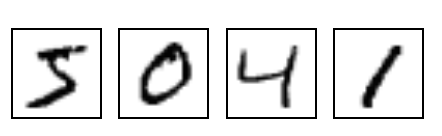
\includegraphics[scale=0.4]{figures/mnist_digits}
\caption{{\bf The MNIST dataset.} Examples of the digits from the handwritten MNIST dataset.}
\label{fig:MNIST}
\end{figure}

Handwritten digit recognition has become one of the standard benchmark problems in the field. Why so? The reason is simple: there exists a very good and freely available data set for it, the MNIST database~\footnote{http://yann.lecun.com/exdb/mnist}, see Fig.~\ref{fig:MNIST}. This curious fact highlights an important aspect of machine learning: it is all about data. The most efficient way to improve machine learning results is to provide more and better data. Thus, one should keep in mind that despite the widespread applications, machine learning is not the hammer for every nail. It is most beneficial if large and \textbf{balanced} data sets, meaning roughly that the algorithm can learn all aspects of the problem equally,  in a machine-readable way are available.

This lecture is an introduction specifically targeting the use of machine learning in different domains of science. In scientific research, we see a vastly increasing number of applications of machine learning, mirroring the developments in industrial technology.
With that, machine learning presents itself as a universal new tool for the exact sciences, standing side-by-side with methods such as calculus, traditional statistics, and numerical simulations. This poses the question, where in the scientific workflow, summerized in Fig.~\ref{fig:scientific_workflow}, these novel methods are best employed.


Once a specific task has been identified, applying machine learning to the sciences does, furthermore, hold its very specific challenges: (i) scientific data has often very particular structure, such as the nearly perfect periodicity in an image of a crystal; (ii) typically, we have specific knowledge about correlations in the data which should be reflected in a machine learning analysis; (iii) we want to understand why a particular algorithm works, seeking a fundamental insight into mechanisms and laws of nature; (iv) in the sciences we are used to algorithms and laws that provide deterministic answers while machine learning is intrinsically probabilistic - there is no absolute certainty. Nevertheless, quantitative precision is paramount in many areas of science and thus a critical benchmark for machine learning methods.
\vspace{10pt}

\begin{figure}
  \centering
  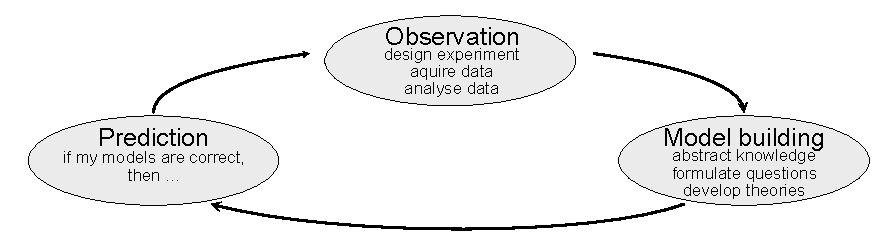
\includegraphics{figures/scientific_workflow}
  \caption{{\bf Simplified scientific workflow.} From observations, via abstraction to building and testing hypothesis or laws, to finally making predictions}
  \label{fig:scientific_workflow}
\end{figure}

\noindent{\bf A note on the concept of a model}\\
In both machine learning and the sciences, models play a crucial role. However, it is important to recognize the difference in meaning: In the natural sciences, a model is a conceptual representation of a phenomenon. A scientific model does not try to represent the whole world, but only a small part of it. A model is thus a simplification of the phenomenon and can be both a theoretical construct, for example the ideal gas model or the Bohr model of the atom, or an experimental simplification, such as a small version of an airplane in a wind channel.

In machine  learning, on the other hand, we most often use a complicated variational function, for example a neural network, to try to approximate a statistical model. But what is a model in statistics? Colloquially speaking, a statistical model comprises a set of statistical assumptions which allow us to calculate the probability $P(x)$ of \emph{any} event $x$. The statistical model does not correspond to the true distribution of all possible events, it simply approximates the distribution.
Scientific and statistical models thus share an important property: neither claims to be a representation of reality.


\subsection{Overview and learning goals}
This lecture is an introduction to basic machine learning algorithms for scientists and students of the sciences.
We will cover
\begin{itemize}
\setlength\itemsep{-0.2em}
    \item the most fundamental machine learning algorithms,
    \item the terminology of the field, succinctly explained,
    \item the principles of supervised and unsupervised learning and why it is so successful,
    \item various architectures of artificial neural networks and the problems they are suitable for,
    \item how we find out what the machine learning algorithm uses to solve a problem.
\end{itemize}

The field of machine learning is full of lingo which to the uninitiated obscures what is at the core of the methods. Being a field in constant transformation, new terminology is being introduced at a fast pace. Our aim is to cut through slang with mathematically precise and concise formulations in order to demystify machine learning concepts for someone with an understanding of calculus and linear algebra.

%All code snippets are expressed in pseudo code for better readability. Several major software packages like pytorch, Keras, tensor flow, Mathematica can be used and have most standard machine learning algorithms implemented.

As mentioned above, data is at the core of most machine learning approaches discussed in this lecture. With raw data in many cases very complex and extremely high dimensional, it is often crucial to first understand the data better and reduce their dimensionality. Simple algorithms that can be used before turning to the often heavy machinery of neural networks will be discussed in the next section, Sec.~\ref{sec:structuring_data}.

The machine learning algorithms we will focus on most can generally be divided into two classes of algorithms, namely \emph{discriminative} and \emph{generative} algorithms as illustrated in Fig.~\ref{fig:overview}. Examples of discriminative tasks include classification problems, such as the aforementioned digit classification or the classification into solid, liquid and gas phases given some experimental observables. Similarly, regression, in other words estimating relationships between variables, is a discriminative problem. More specifically, we try to approximate the conditional probability distribution $P(y|x)$ of some variable $y$ (the label) given some input data $x$. As data is provided in the form of input and target data for most of these tasks, these algorithms usually employ supervised learning. Discriminative algorithms are most straight-forwardly applicable in the sciences and we will discuss them in Secs.~\ref{sec: linear methods for supervised learning} and \ref{sec:supervised}.
%~\ref{chap:noneuralnetworks} and \ref{chap:neuralnetworks}.

\begin{figure}
  \centering
  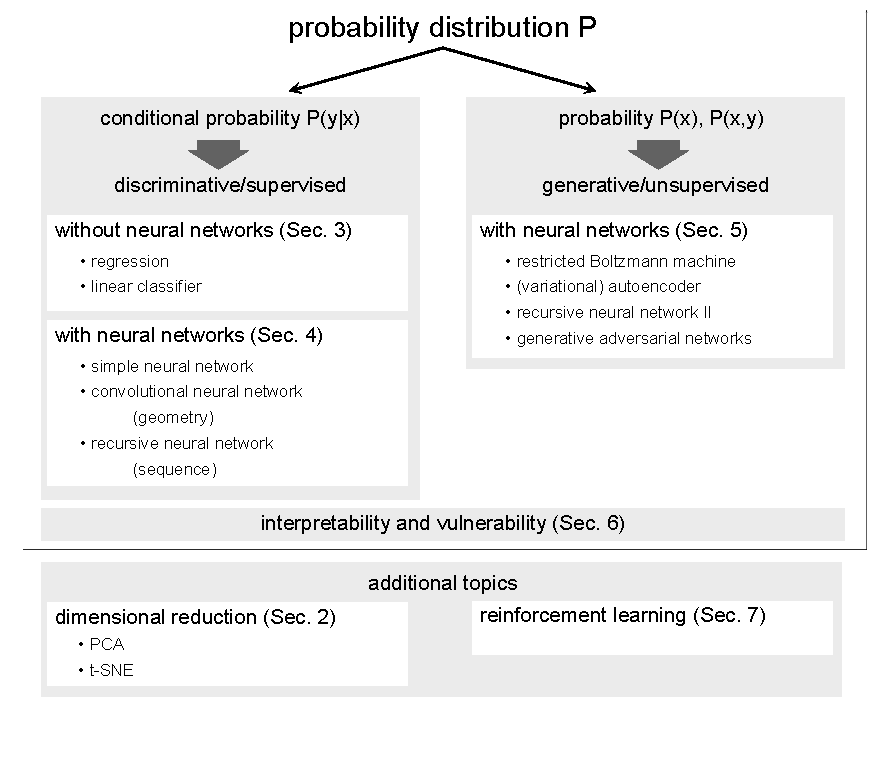
\includegraphics{figures/overview}
  \caption{Overview over the plan of the lecture from the perspective of learning probability distributions.}
  \label{fig:overview}
\end{figure}


Generative algorithms, on the other hand, model a probability distribution $P(x)$. These approaches are---once trained---in principle more powerful, since we can also learn the joint probability distribution $P(x,y)$ of both the data $x$ and the labels $y$ and infer the conditional probability of $y$. Still, the more targeted approach of discriminative learning is better suited for many problems. However, generative algorithms are useful in the natural sciences, as we can sample from a known probability distribution, for example for image denoising, or when trying to find new compounds/molecules resembling known ones with given properties. These algorithms are discussed in Sec.~\ref{sec:unsupervised}.
%\ref{chap:unsupervised}.

The promise of artificial \emph{intelligence} may trigger unreasonable expectations in the sciences. After all,  scientific knowledge generation is one of the most complex intellectual processes.
%starting from observations, via abstraction to building and testing hypothesis or laws, to finally making predictions. 
Computer algorithms are certainly far from achieving anything on that level of complexity and will in the near future not formulate new laws of nature independently. Nevertheless, researchers study how machine learning can help with individual segments of the scientific workflow (Fig.~\ref{fig:scientific_workflow}).
While the type of abstraction needed to formulate Newton's laws of classical mechanics seems incredibly complex, neural networks are very good at \emph{
implicit knowledge representation}. To understand precisely how they achieve certain tasks, however, is not an easy undertaking. We will discuss this question of \emph{interpretability} in Sec.~\ref{sec:interpretability}.
%\ref{chap: Interpretability}.


A third class of algorithms, which does not neatly fit the framework of approximating a statistical model and thus the distinction into discriminative and generative algorithms is known as reinforcement learning. Instead of approximating a statistical model, reinforcement learning tries to optimize strategies (actions) for achieving a given task. Reinforcement learning has gained a lot of attention with Google's AlphaGo Zero, a computer program that beat the best Go players in the world. As an example for an application in the sciences, reinfocrment learning can be used to decide on what experimental configuration to perform next. While the whole topic is beyond the scope of this lecture, we will give an introduction to the basic concepts of reinforcement learning in Sec.~\ref{sec:RL}.


A final note on the practice of learning. While the machine learning machinery is extremely powerful, using an appropriate architecture and the right training details, captured in what are called \emph{hyperparameters}, is crucial for its successful application. Though there are attempts to learn a suitable model and all hyperparameters as part of the overall learning process, this is not a simple task and requires immense computational resources. A large part of the machine learning success is thus connected to the experience of the scientist using the appropriate algorithms. 
We thus strongly encourage solving the accompanying exercises carefully and taking advantage of the exercise classes.

%Often, what is behind the lingo has a clear mathematical meaning. One goal of this book is to clarify this meaning and thus reduce the aforementioned barrier. For instance:
%\begin{itemize}
%    \item An \emph{\index{neuron}}\emph{artificial neuron} is a function that maps a real vector to a real number. It performs the scalar product with a constant (weight) vector and then applies a non-linear function to the result. This form is inspired by neurons in the brain that are connected via synapses to other neurons. If a signal arriving through the synapses is larger than some threshold, the neuron ``fires'' and transmits it further. The perceptron mimics this behaviour.
%   \item The \emph{layers} of a neural network refer to the successive applications, in other words nesting, of certain functions.
 %   \german{
 %   Die \emph{\index{Schichten}} Schichten (auch Lagen) eines neuronalen Netzwerks beschreiben die aufeinanderfolgende Anwendung von verscheidenen Funktionen. 
 %   }
%    \item \emph{(Feed-forward) \index{neural networks}} are most fundamentally a class of variational functions, i.e., functions that depend on some parameters. They have a layered structure, and the function represented by each layer has a fixed form, up to the choice of the parameters.
%    \item \emph{Learning} refers to the parameter optimization of the variatonal function to perform a given task, such as classification or regression. This optimization is typically performed using some form of gradient descent.
%    \item The \emph{backpropagation algorithm} is, at its heart, the chain rule of differentiation. It helps to minimize the computational cost for the gradiant descent, in other words for computing the change in the function value, when the variational parameters (in a given layer) are varied.
%\end{itemize}
%Note that here, and throughout this book, we {\it emphasize} the terminology that we introduce.

\subsection{Resources}
While it may seem that implementing ML tasks is computationally challenging, actually almost any ML task one might be interested in can be done with relatively few lines of code simply by relying on external libraries or mathematical computing systems such as Mathematica or Matlab. At the moment, most of the external libraries are written for the Python programming language.
Here are some useful Python libraries:
\begin{enumerate}
    \item \textbf{TensorFlow.} Developed by Google, Tensorflow is one of the most popular and flexible library for machine learning with complex models, with full GPU support.
    \item \textbf{PyTorch.} Developed by Facebook, Pytorch is the biggest rival library to Tensorflow, with pretty much the same functionalities.
    \item \textbf{Scikit-Learn.} Whereas TensorFlow and PyTorch are catered for deep learning practitioners, Scikit-Learn provides much of the traditional machine learning tools, including linear regression and PCA.
    \item \textbf{Pandas.} Modern machine learning is largely reliant on big datasets. This library provides many helpful tools to handle these large datasets.
\end{enumerate}

\subsection{Prerequisites}
This course is aimed at students of the (natural) sciences with a basic mathematics education and some experience in programming. In particular, we assume the following prerequisites:
\begin{itemize}
  \item Basic knowledge of calculus and linear algebra.
  \item Rudimentary knowledge of statistics and probability theory (advantageous).
  \item Basic knowledge of a programming language. For the teaching assignments, you are free to choose your preferable one. The solutions will typically be distributed in Python in the form of Jupyter notebooks.
\end{itemize}
Please, don't hesitate to ask questions if any notions are unclear.

\subsection{References}
For further reading, we recommend the following books:
\begin{itemize}
	\item {\bf ML without neural networks}: \emph{The Elements of Statistical Learning}, T. Hastie, R. Tisbshirani, and J. Friedman (Springer)
	\item {\bf ML with neural networks}: \emph{Neural Networks and Deep Learning}, M. Nielson (\href{http://neuralnetworksanddeeplearning.com}{http://neuralnetworksanddeeplearning.com})
	\item {\bf Deep Learning Theory}: \emph{Deep Learning}, I. Goodfellow, Y. Bengio and A. Courville (\href{http://www.deeplearningbook.org}{http://www.deeplearningbook.org})
	\item {\bf Reinforcement Learning}: \emph{Reinforcement Learning}, R. S. Sutton and A. G. Barto (MIT Press)
\end{itemize}
